\documentclass{article}

\usepackage{amsmath}
\usepackage{amssymb}
\usepackage{tikz}
\usetikzlibrary{shapes,arrows,positioning}
\renewcommand{\thesubsection}{\thesection \space \alph{subsection})}

\title{Planing, Learning and Intelligent Decision Making - Homework 2}
\author{99326 - Sebastião Carvalho, 99331 - Tiago Antunes}
\date{\today}

\begin{document}

\maketitle

\tableofcontents

\section{Question 1}

\subsection{}

Using $\mathbb{X}$ as the state space, $\mathbb{X} = \{ A, B, C\}$.

\bigskip

The transition matrix is given by
$
\begin{bmatrix}
    0 & 1 & 0 \\
    0.5 & 0 & 0.5 \\
    1 & 0 & 0
\end{bmatrix}
$.

\bigskip

Where the first row represents the transition probabilities from state A, the second row from state B and the third row from state C.
Each column represents the transition probabilities to state A, B and C, respectively.

\bigskip

The diagram of the Markov chain is given by

\begin{figure}
    \centering
    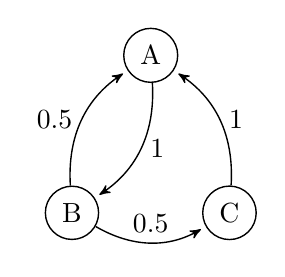
\begin{tikzpicture}[->,>= stealth',shorten >=2pt, line width =0.5 pt ,
node distance=2 cm]
        \node [circle, draw] (A) at (0,0) {A};
        \node [circle, draw] (B) at (-1, -2) {B};
        \node [circle, draw] (C) at (1, -2) {C};
        \path (A) edge [bend left] node [right] {$1$} (B);
        \path (B) edge [bend left] node [left] {$0.5$} (A);
        \path (B) edge [bend right] node [above] {$0.5$} (C);
        \path (C) edge [bend right] node [right] {$1$} (A);
    \end{tikzpicture}
    \caption{Markov Chain}
    \label{fig: markov_chain}
\end{figure}


\subsection{}

For state A, we have 2 possible paths to reach state A again, $A \rightarrow B \rightarrow A$ and 
$A \rightarrow B \rightarrow C \rightarrow A$. With the transition matrix, we can calculate the probability of each path.

\bigskip

Using $x_t$ to represent the state at time t. 

The probability of the first path is $P(x_1=B|x_0=A) * P(x_2=A|x_1=B) = 1 * 0.5 = 0.5.$

The probability of the second path is $P(x_1=B|x_0=A) * P(x_2=C|x_1=B) * P(x_3=A|x_2=C) = 1 * 0.5 * 1 = 0.5.$


Since the first path takes 2 steps and the second path takes 3 steps, 
$T_{AA} = 0.5 * 2 + 0.5 * 3 = 2.5$.

For state B, we have 2 possible paths to reach state B again, $B \rightarrow A \rightarrow B$ and
$B \rightarrow C \rightarrow A \rightarrow B$. With the transition matrix, we can calculate the probability of each path.

The probability of the first path is $P(x_1=A|x_0=B) * P(x_2=B|x_1=A) = 0.5 * 1 = 0.5.$
The probability of the second path is $P(x_1=C|x_0=B) * P(x_2=A|x_1=C) * P(x_3=B|x_2=A) = 0.5 * 1 * 1 = 0.5.$

Since the first path takes 2 steps and the second path takes 3 steps,
$T_{BB} = 0.5 * 2 + 0.5 * 3 = 2.5$.

For state C, we have infinite possible paths to reach state C again, since it the bot can stay in states A and B indefinitely.

The shortest path is $C \rightarrow A \rightarrow B \rightarrow C$, with 3 steps.
The probability of this path is $P(x_1=A|x_0=C) * P(x_2=B|x_1=A) * P(x_3=C|x_2=B) = 1 * 0.5 * 1 = 0.5$.

The second shortest path is $C \rightarrow A \rightarrow B \rightarrow A \rightarrow B \rightarrow C$, with 5 steps.
The probability of this path is $P(x_1=A|x_0=C) * P(x_2=B|x_1=A) * P(x_3=A|x_2=B) * P(x_4=B|x_3=A) * P(x_5=C|x_4=B) 
= 1 * 1 * 0.5 * 1 * 0.5 = 0.25$.


To calculate the average number of steps, we need to calculate $\sum_{n=1}^{\infty} (2n + 1) / 2^n = 5$. % TODO : Explain the sum

Where 2n + 1 is the number of steps and 1/2n is the probability of the path. n represents the number of times we arrive at 
state B.

With this, $T_{CC} = 5$.



\subsection{}

\end{document}